\chapter{快速使用指南}
\label{ch:quick-start}

\textbf{本章将通过多个小节,介绍如何快速
成功编译出一份符合学校要求的毕业论文。}

其中,\autoref{sec:local-compile}介绍在本地电脑上编译生成 PDF;
\autoref{sec:overleaf-compile}介绍在 Overleaf(浏览器)上编译生成 PDF。这两种方法相互独立,你可以根据喜好自行选择其中一种。

\section{方法一:在本地电脑上编译生成 PDF}
\label{sec:local-compile}

\subsection{安装 TeX 发行版——TeX Live}

访问 \href{https://tug.org/texlive/}{tug.org/texlive},下载并安装 TeX Live。TeX Live 包含了所有将 \LaTeX 编译成 PDF 所需的代码和工具。

\begin{itemize}[nosep]
  \item \textbf{Windows}
  
  参考 \href{https://www.tug.org/texlive/windows.html#install}{Easy install},下载并运行 \href{https://mirror.ctan.org/systems/texlive/tlnet/install-tl-windows.exe}{\texttt{install-tl-windows.exe}}。
  
  \item \textbf{Linux}
  
  参考 \href{https://www.tug.org/texlive/quickinstall.html}{Quick install},下载 \href{https://mirror.ctan.org/systems/texlive/tlnet/install-tl-unx.tar.gz}{\texttt{install-tl-unx.tar.gz}} 并解压,运行 \texttt{install-tl}。
  
  \item \textbf{macOS}
  
  参考 \href{https://www.tug.org/mactex/mactex-download.html}{Downloading MacTeX},下载并运行 \href{https://mirror.ctan.org/systems/mac/mactex/MacTeX.pkg}{\texttt{MacTeX.pkg}}。
\end{itemize}

\begin{figure}[H]
  \begin{center}
    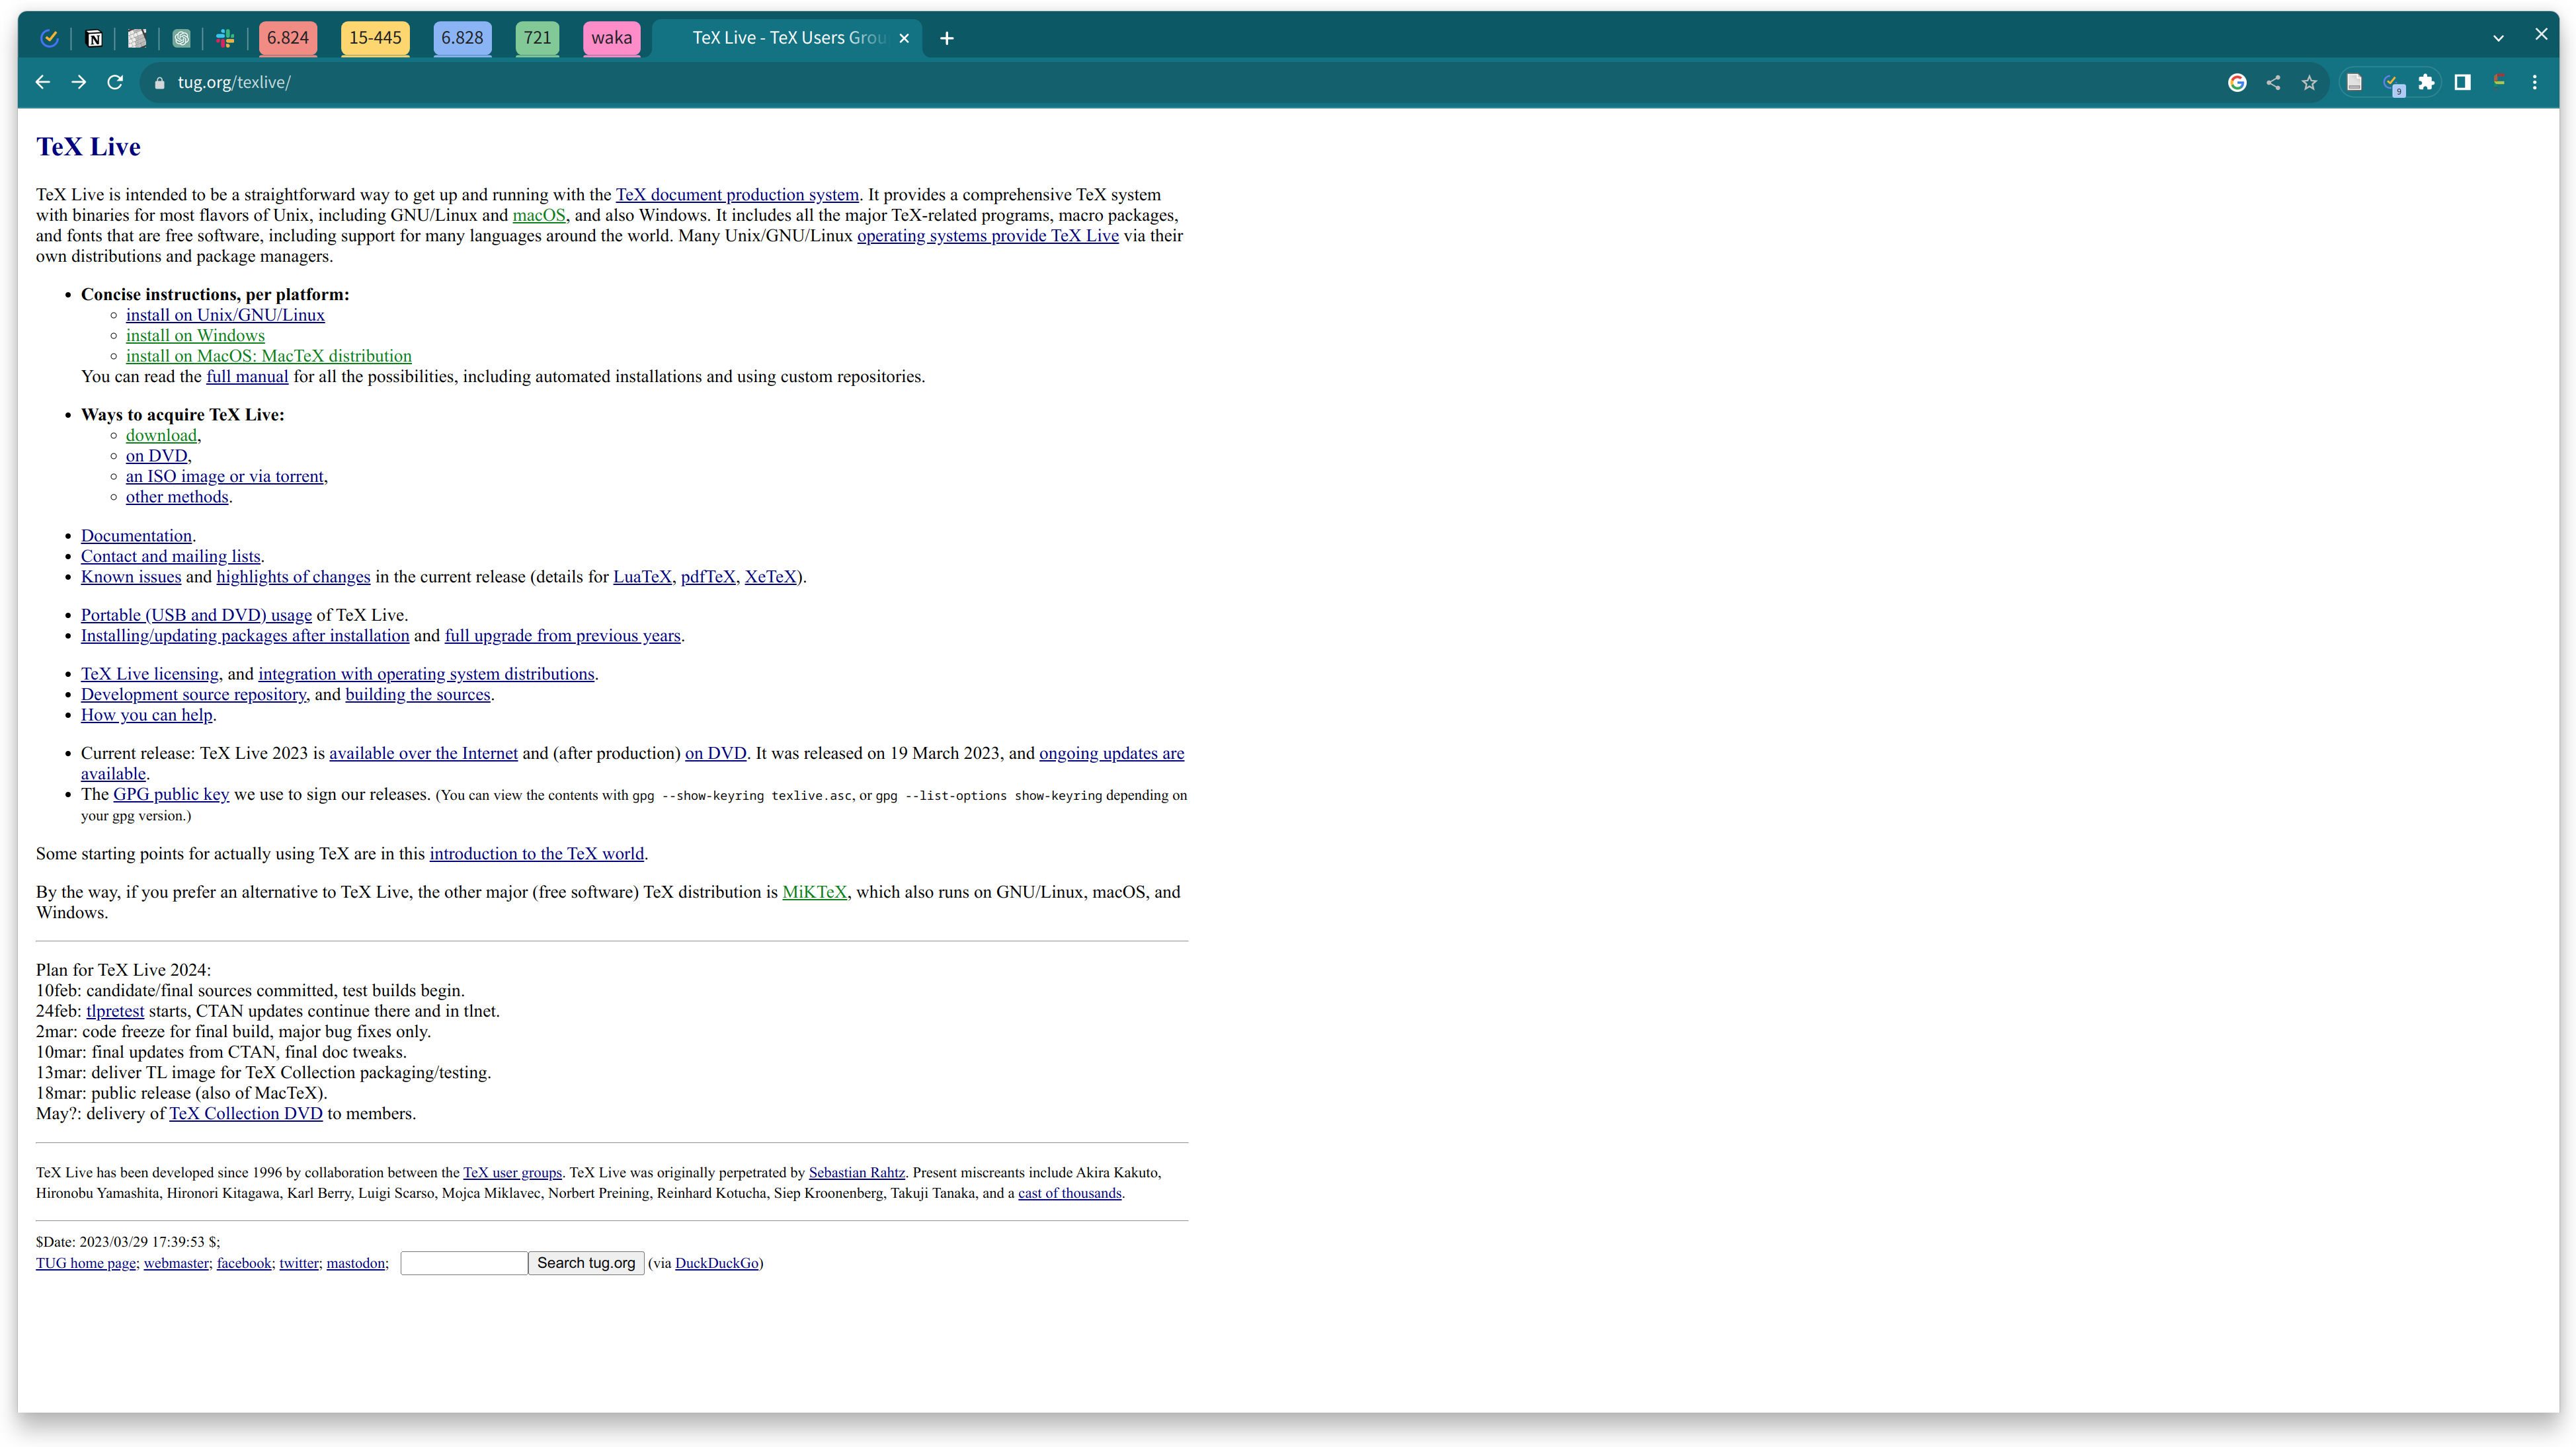
\includegraphics[width=0.85\textwidth]{imgs/local-texlive-download.png}
  \end{center}
  \caption{TeX Live 下载页面}
  \label{fig:local-texlive-download}
\end{figure}

\clearpage
\subsection{安装编辑器——TeXstudio}

访问 \href{https://texstudio.org}{texstudio.org},下载并安装 TeXstudio。TeXstudio 是一个开源的、跨平台的、功能强大的 \LaTeX 编辑器。使用它,你可以更方便地进行 \LaTeX 的写作与编辑。

\begin{figure}[H]
  \begin{center}
    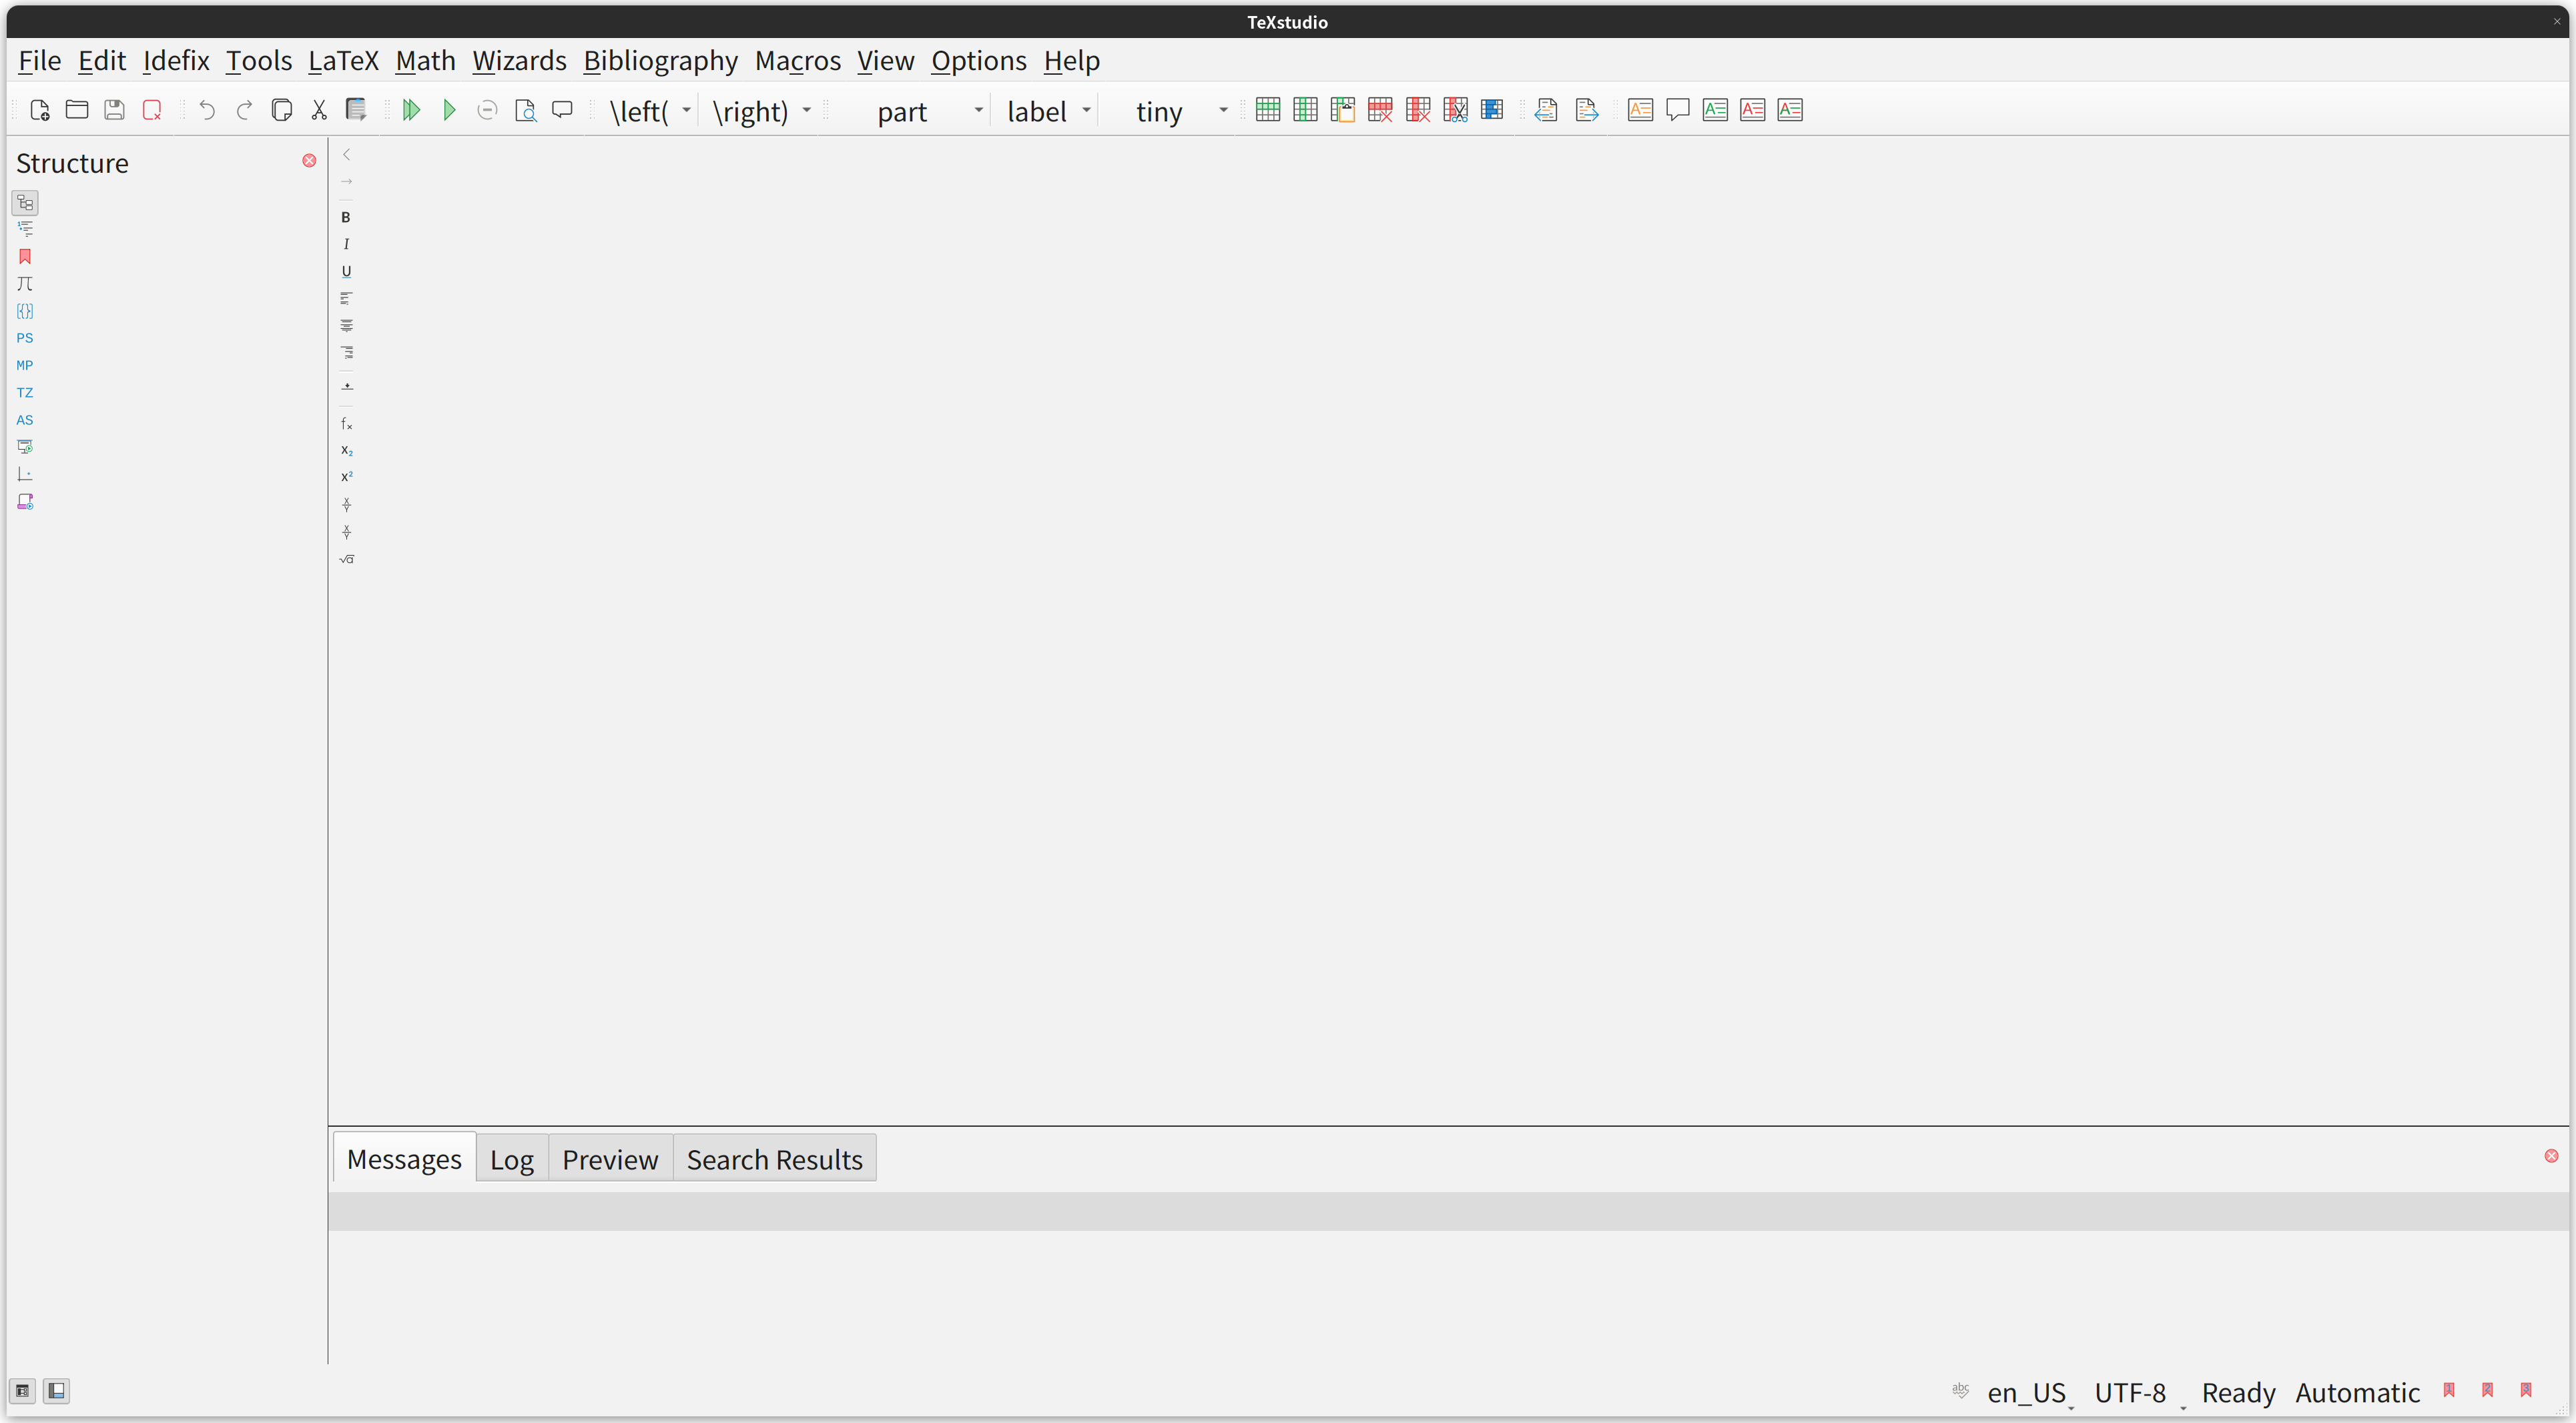
\includegraphics[width=0.85\textwidth]{imgs/texstudio-overview.png}
  \end{center}
  \caption{TeXstudio 界面}
  \label{fig:texstudio-overview}
\end{figure}

\subsection{下载最新模板} \label{sec:download}

\textit{如果你选择使用目前版本的模板,可以跳过该步骤。}

访问 \href{https://bithesis.bitnp.net/guide/downloading-using-templates.html#下载模板包并解压}{BIThesis.bitnp.net → 下载模板},按照网页提示,从\href{https://mirror.bit.edu.cn/github-release/BITNP/BIThesis/LatestRelease/}{校内开源镜像站}或\href{https://github.com/BITNP/BIThesis/releases/latest}{校外 GitHub Releases}
下载模板压缩包\isGraduateTF{``graduate-thesis.zip''}{``undergraduate-thesis.zip''}。

\isGraduateTF{}{
  \textit{若为全英文专业,请选择``undergraduate-thesis-en.zip''。}
}

\begin{figure}[H]
  \begin{center}
    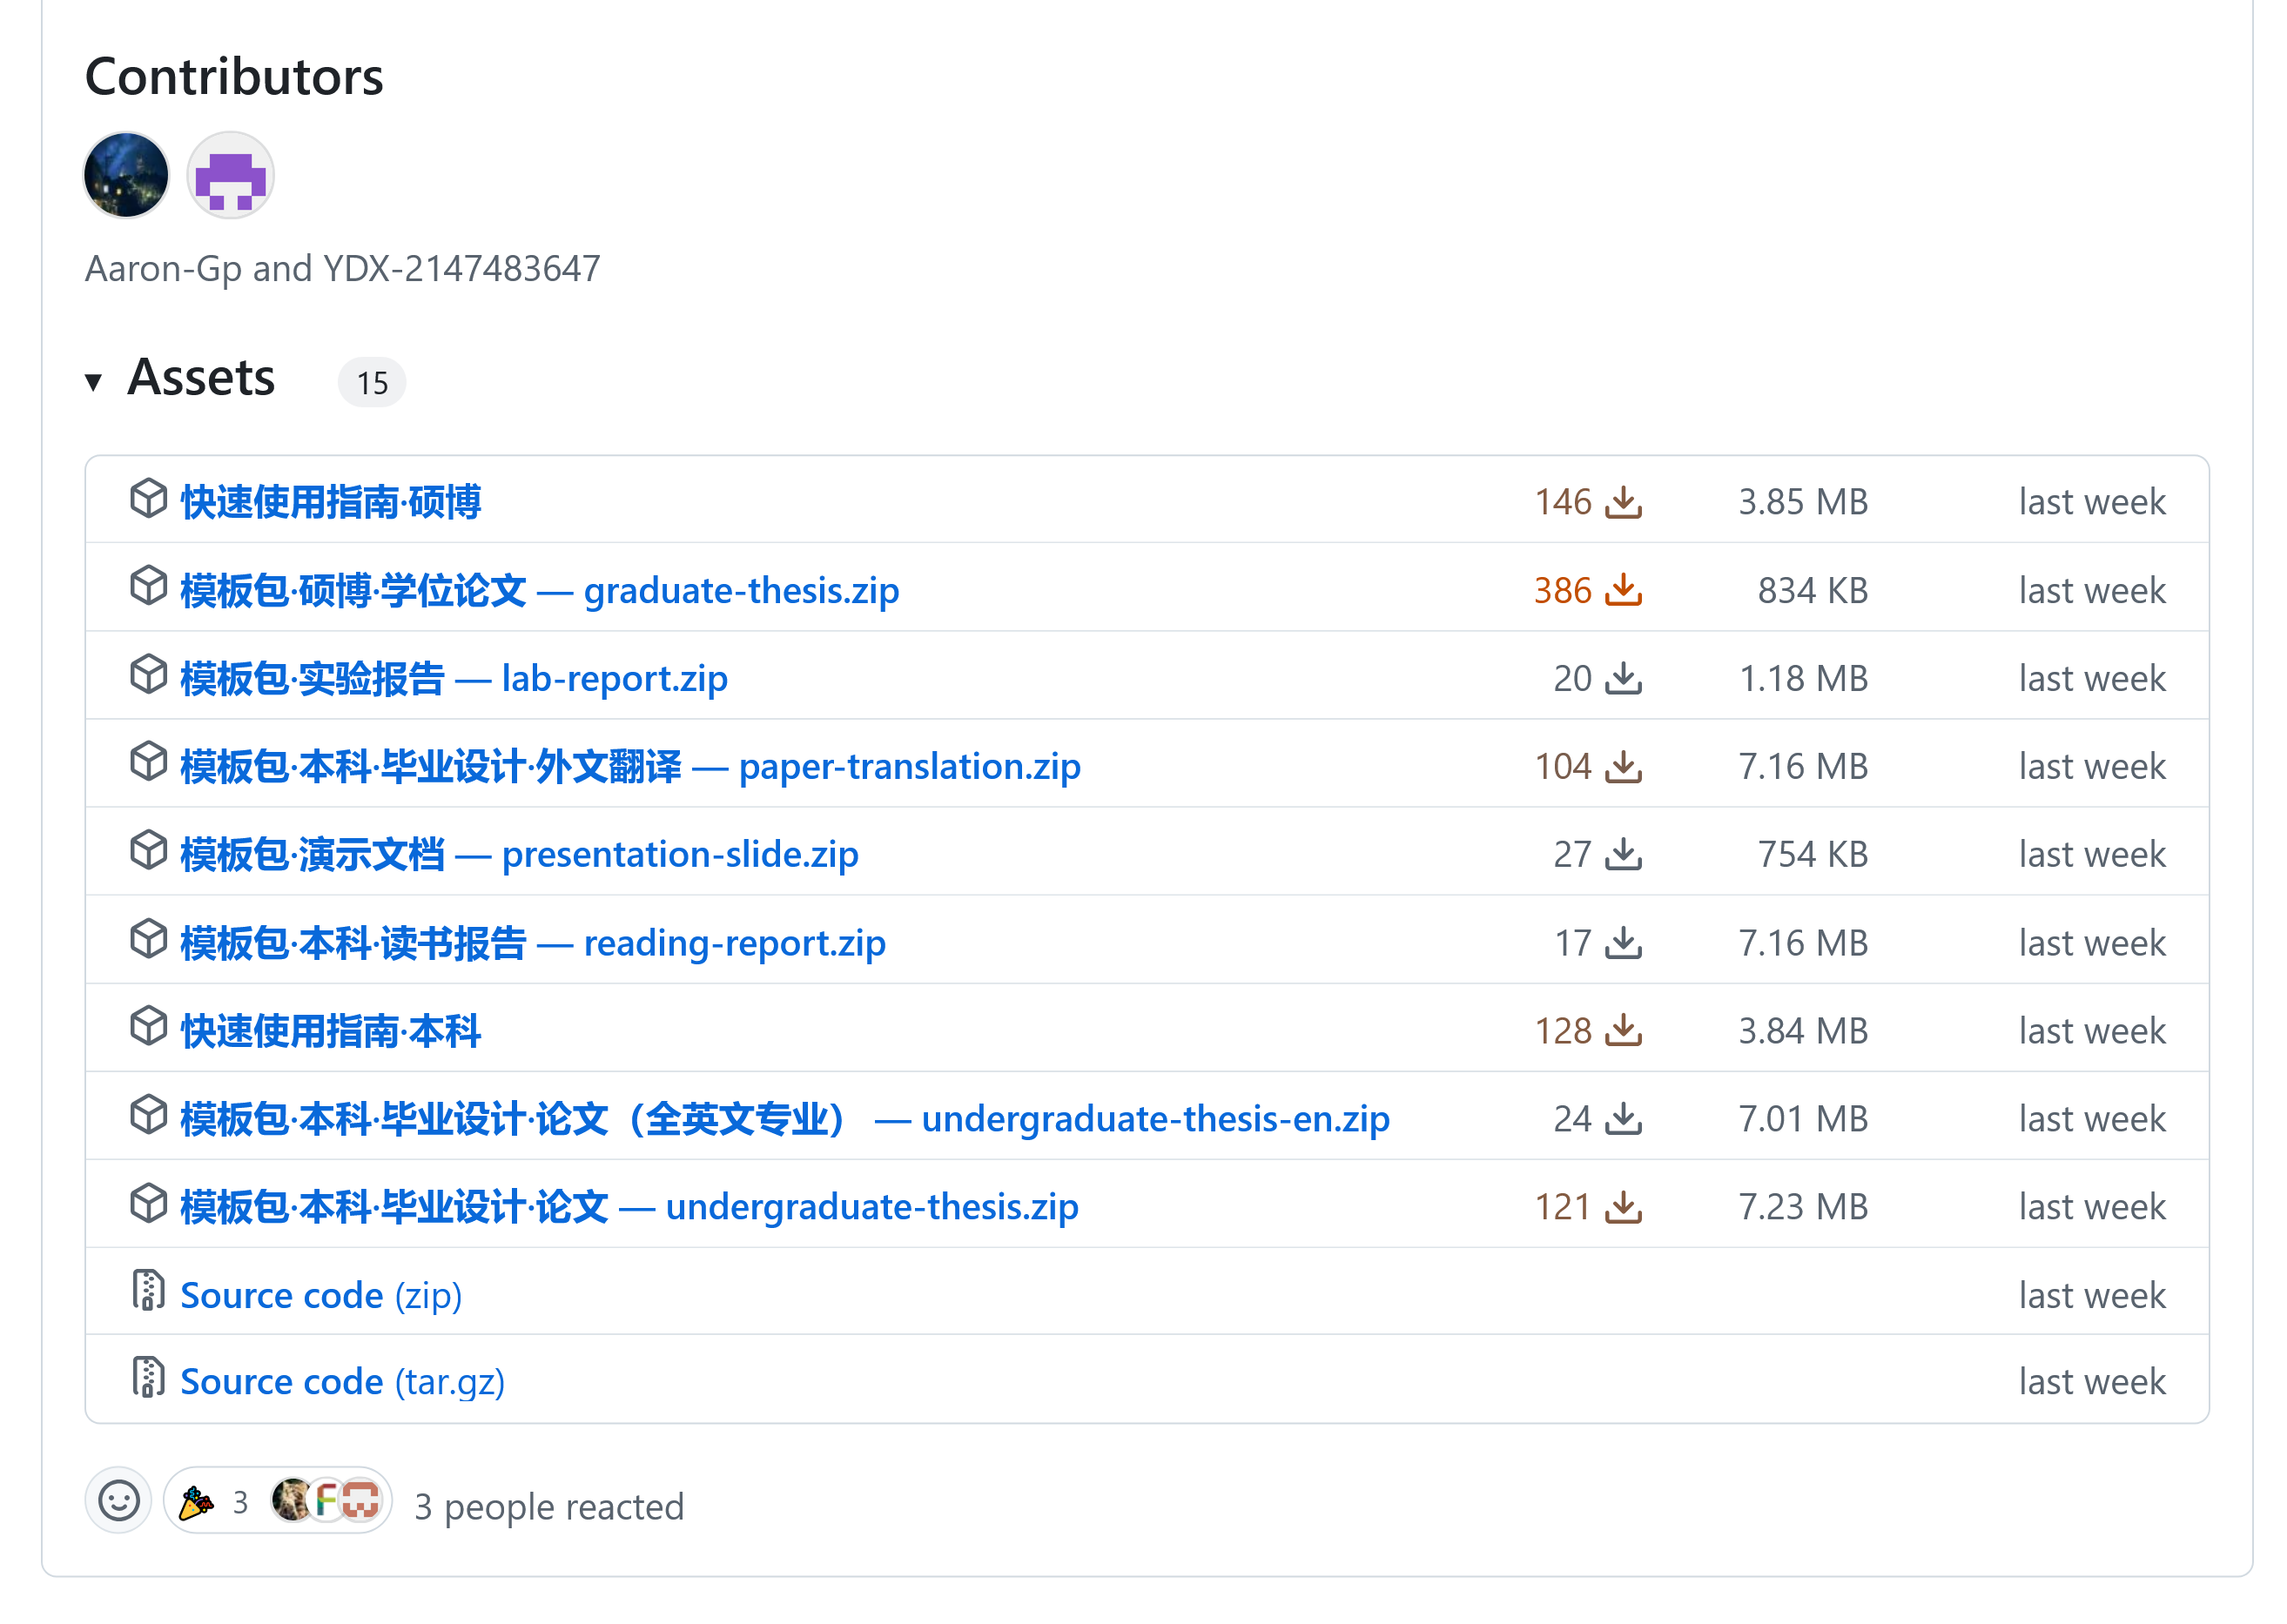
\includegraphics[width=0.6\textwidth]{imgs/github-releases.png}
  \end{center}
  \caption{校外 GitHub Releases 模板下载页面}
  \label{fig:local-template-download}
\end{figure}

\clearpage
\subsection{编译生成 PDF}

解压模板压缩包,打开 TeXstudio,点击 ``File → Open'' 按钮,选择 ``main.tex'' 文件,即可打开模板。

接着,点击 ``Build \& View'' 按钮(两个叠加的绿色三角),即可编译生成 PDF。

\begin{figure}[H]
  \begin{center}
    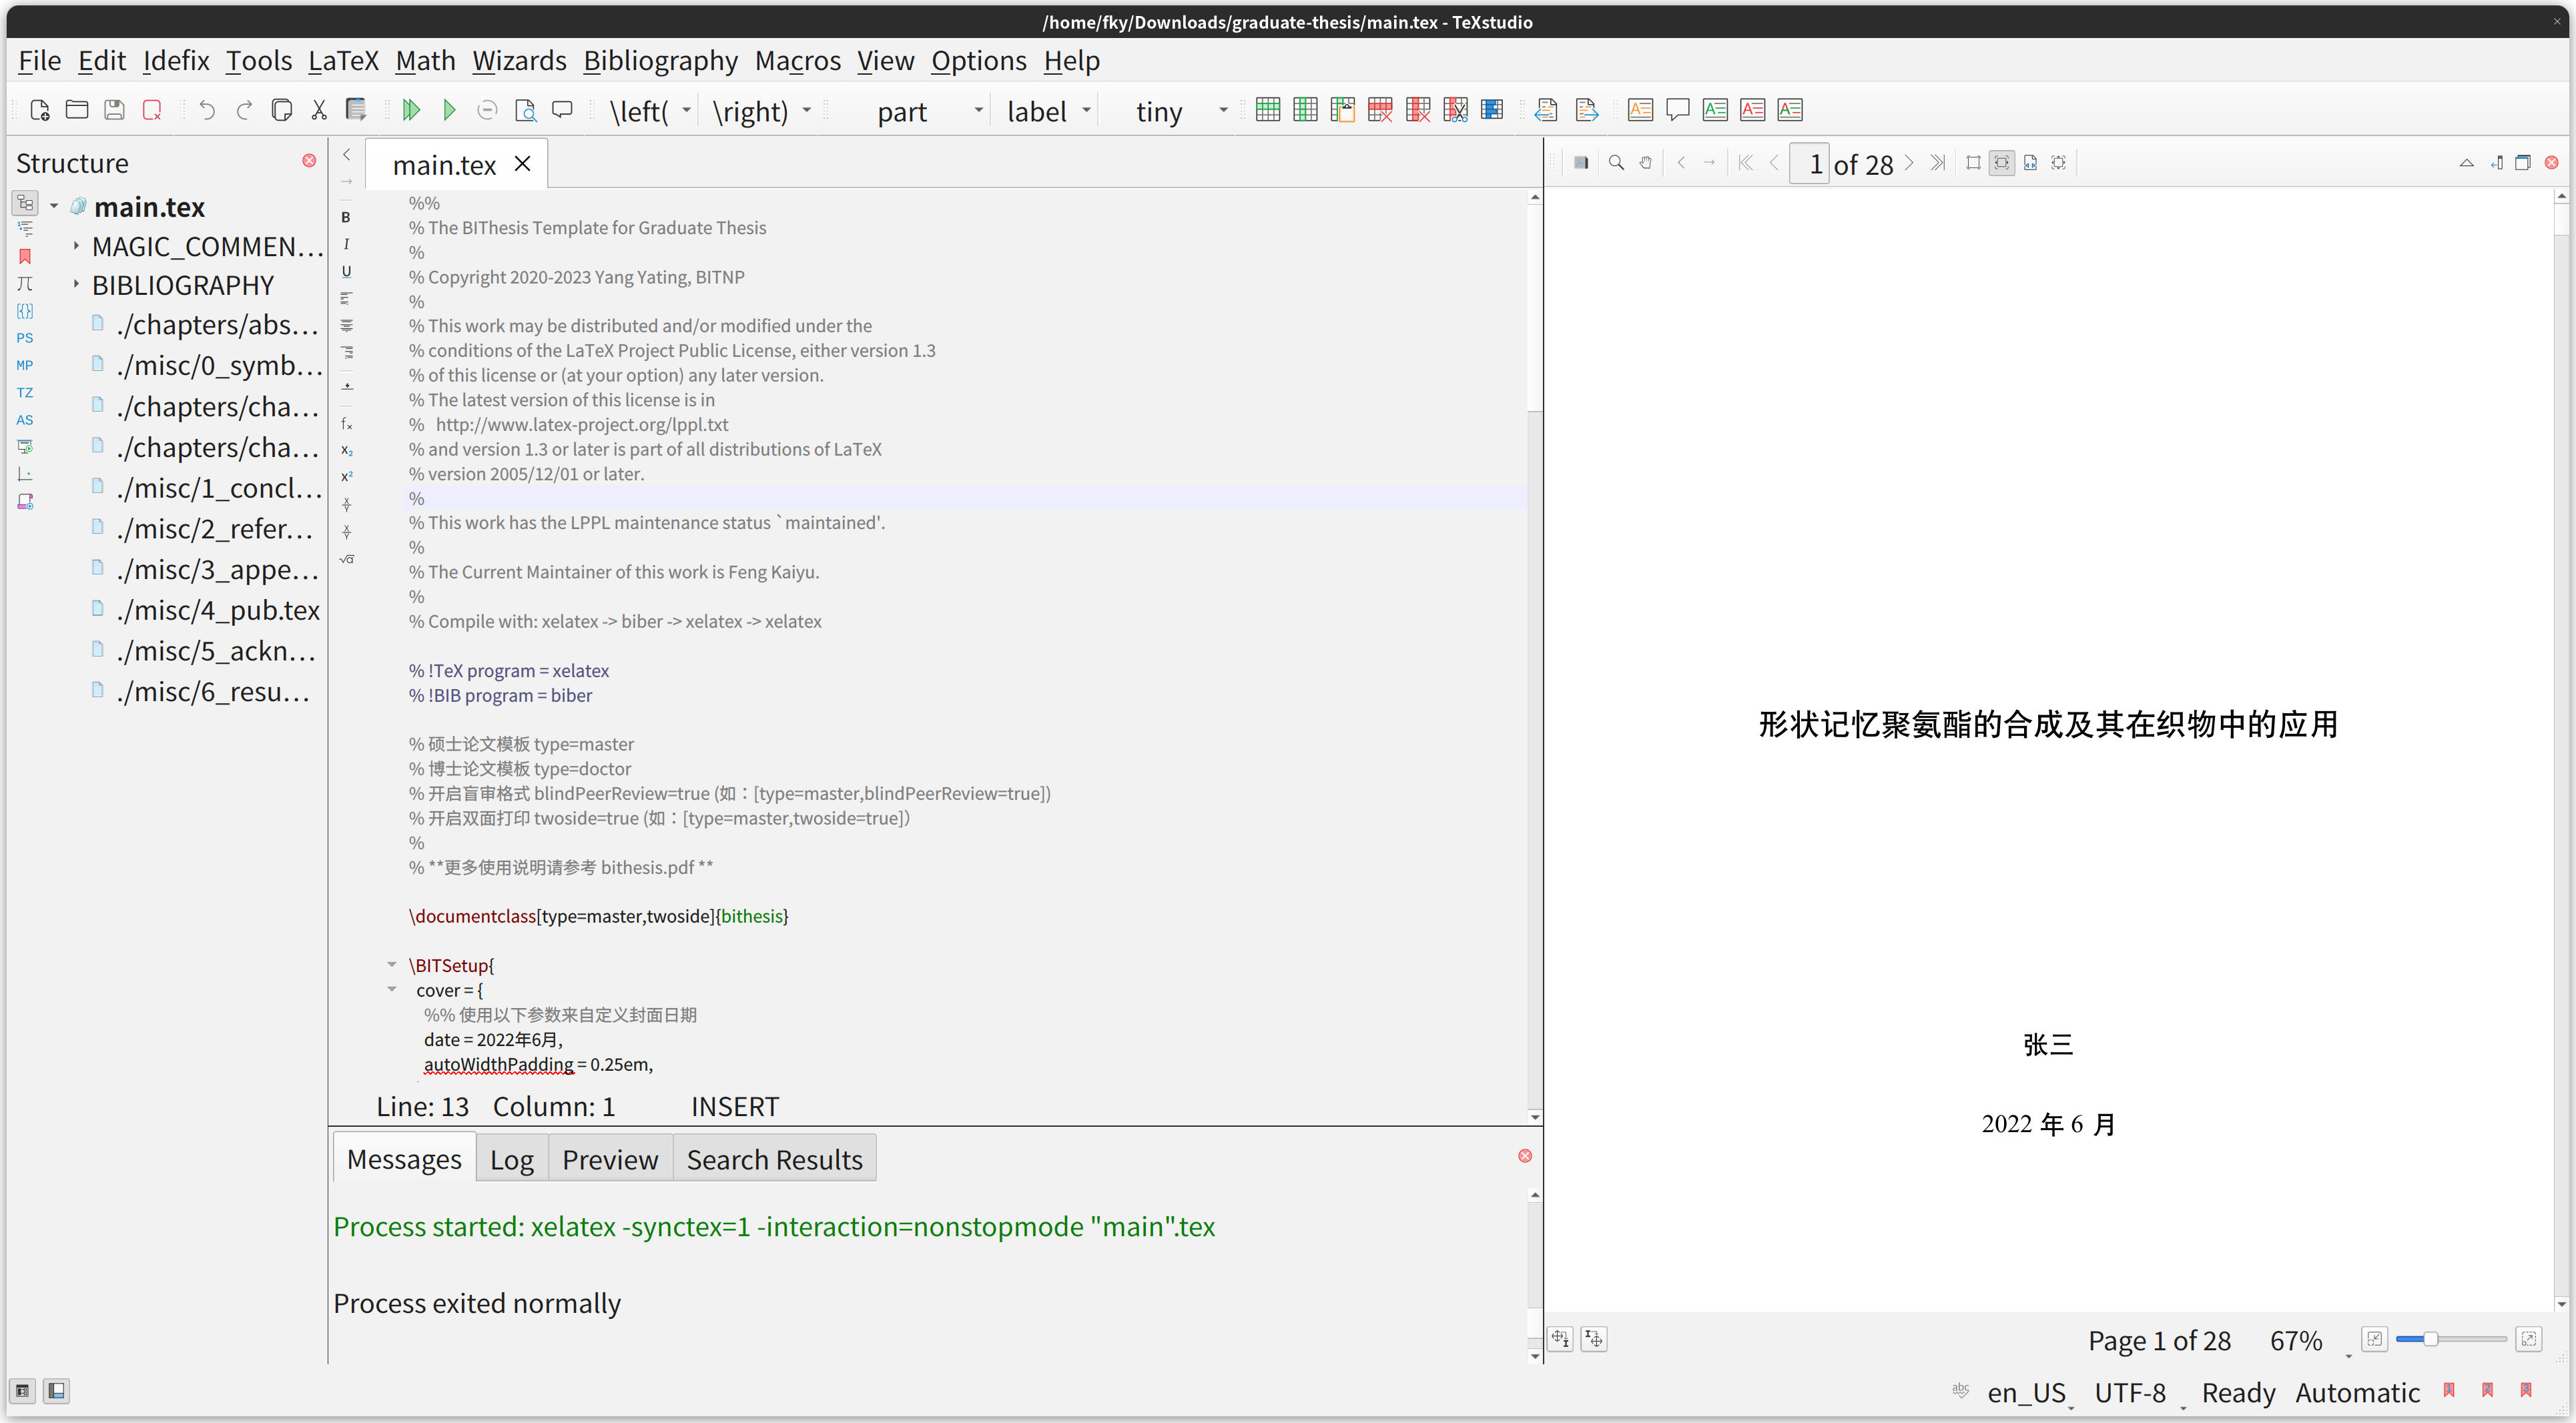
\includegraphics[width=0.85\textwidth]{imgs/texstudio-compile-and-view.png}
  \end{center}
  \caption{TeXstudio 编译生成 PDF}
  \label{fig:texstudio-compile-and-view}
\end{figure}

\clearpage
\section{方法二:在 Overleaf(浏览器)上编译生成 PDF}
\label{sec:overleaf-compile}

\BIThesis 项目已经在 Overleaf 上分享了多个模板,它们
会与最新版本保持同步\footnote{需要注意,你复制的模板不会自动更新。}。
因此,你可以直接在 Overleaf 上复制并使用这些模板。

\vspace{\fill}
\subsection{注册 Overleaf 账号}

访问 \href{https://cn.overleaf.com}{overleaf.com}(如\autoref{fig:overleaf-register}所示),点击右上角的 ``Register'' 按钮,注册账号并登录。

\begin{figure}[H]
  \begin{center}
    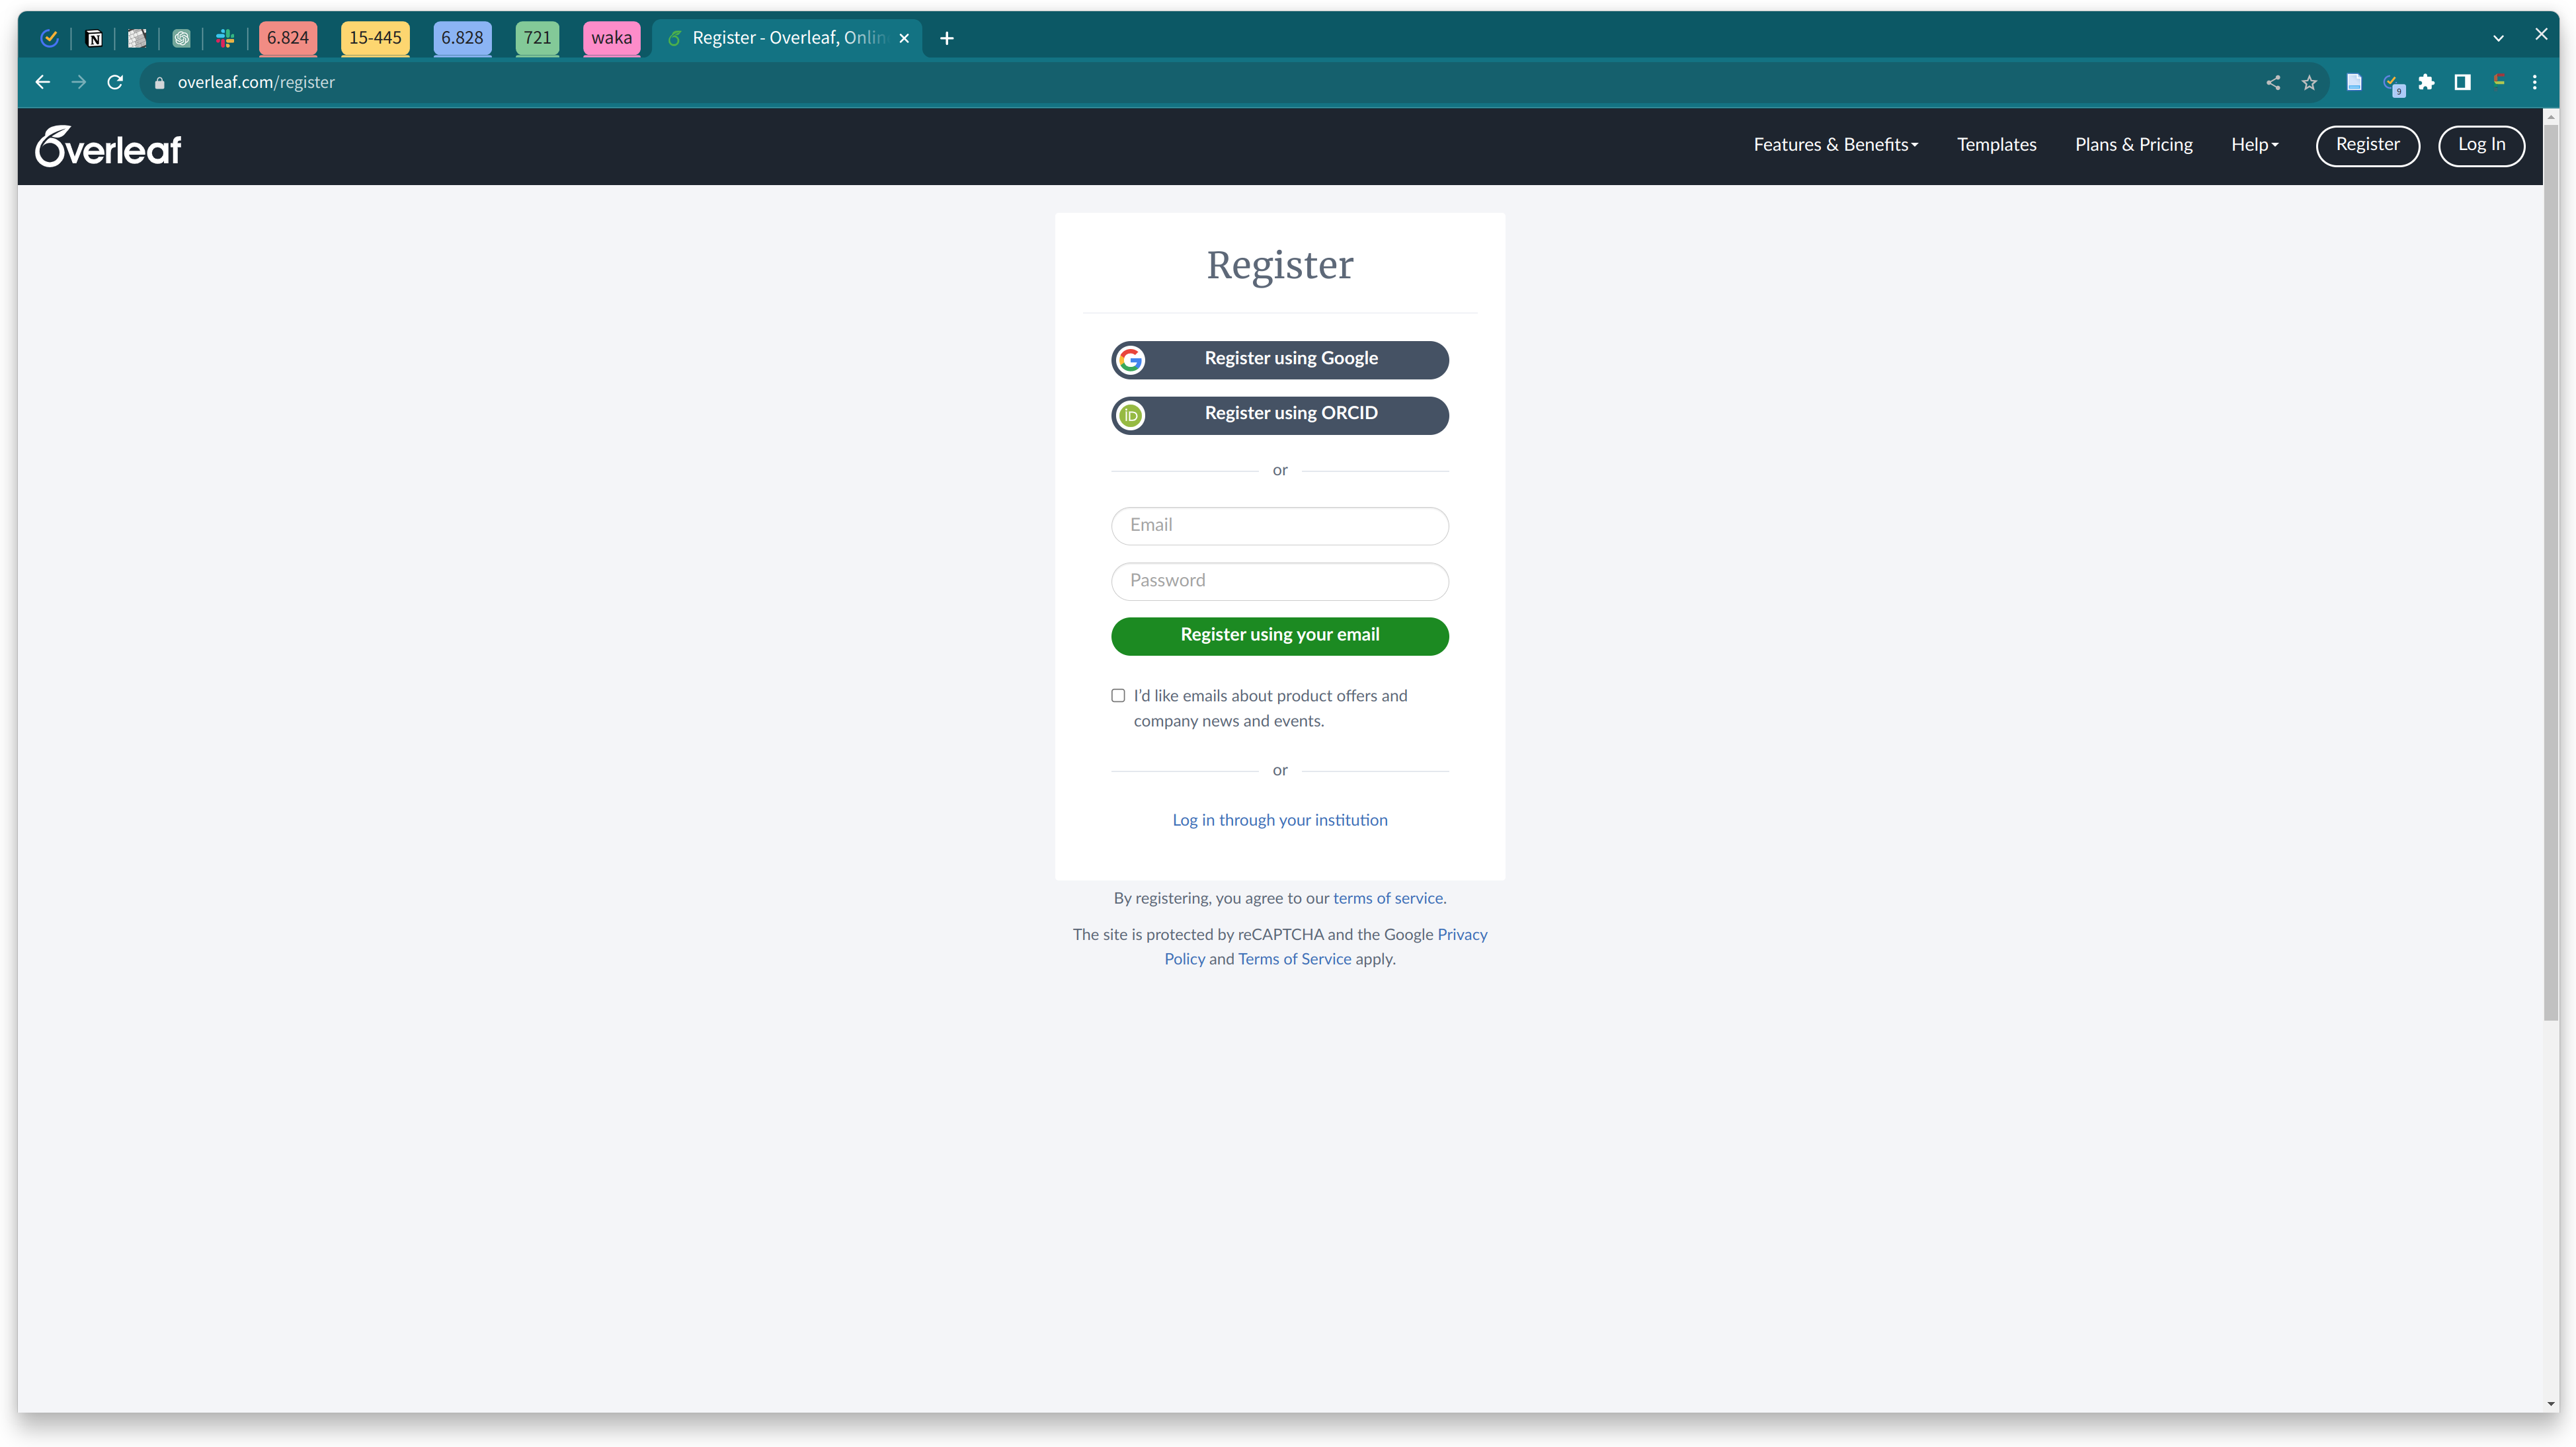
\includegraphics[width=0.85\textwidth]{imgs/overleaf-register.png}
  \end{center}
  \caption{Overleaf 注册页面}
  \label{fig:overleaf-register}
\end{figure}

\vspace{\fill}
\subsection{访问 \BIThesis 的 Overleaf 模板}

访问 \href{https://bithesis.bitnp.net/guide/preface.html#q-bithesis-都包含哪些模板}{BIThesis.bitnp.net →(右上角)Overleaf},即可跳转到模板页面。

找到\isGraduateTF{“研究生·学位论文”}{“本科生·毕业设计·论文”}模板,点击 ``open in Overleaf'' 按钮,即可跳转到 Overleaf 上分享的项目中。

\isGraduateTF{}{
  \textit{若为全英文专业,请选择“本科生·毕业设计·论文(全英文专业)”。}
}

\vspace{\fill}
\clearpage

\begin{figure}[H]
  \begin{center}
    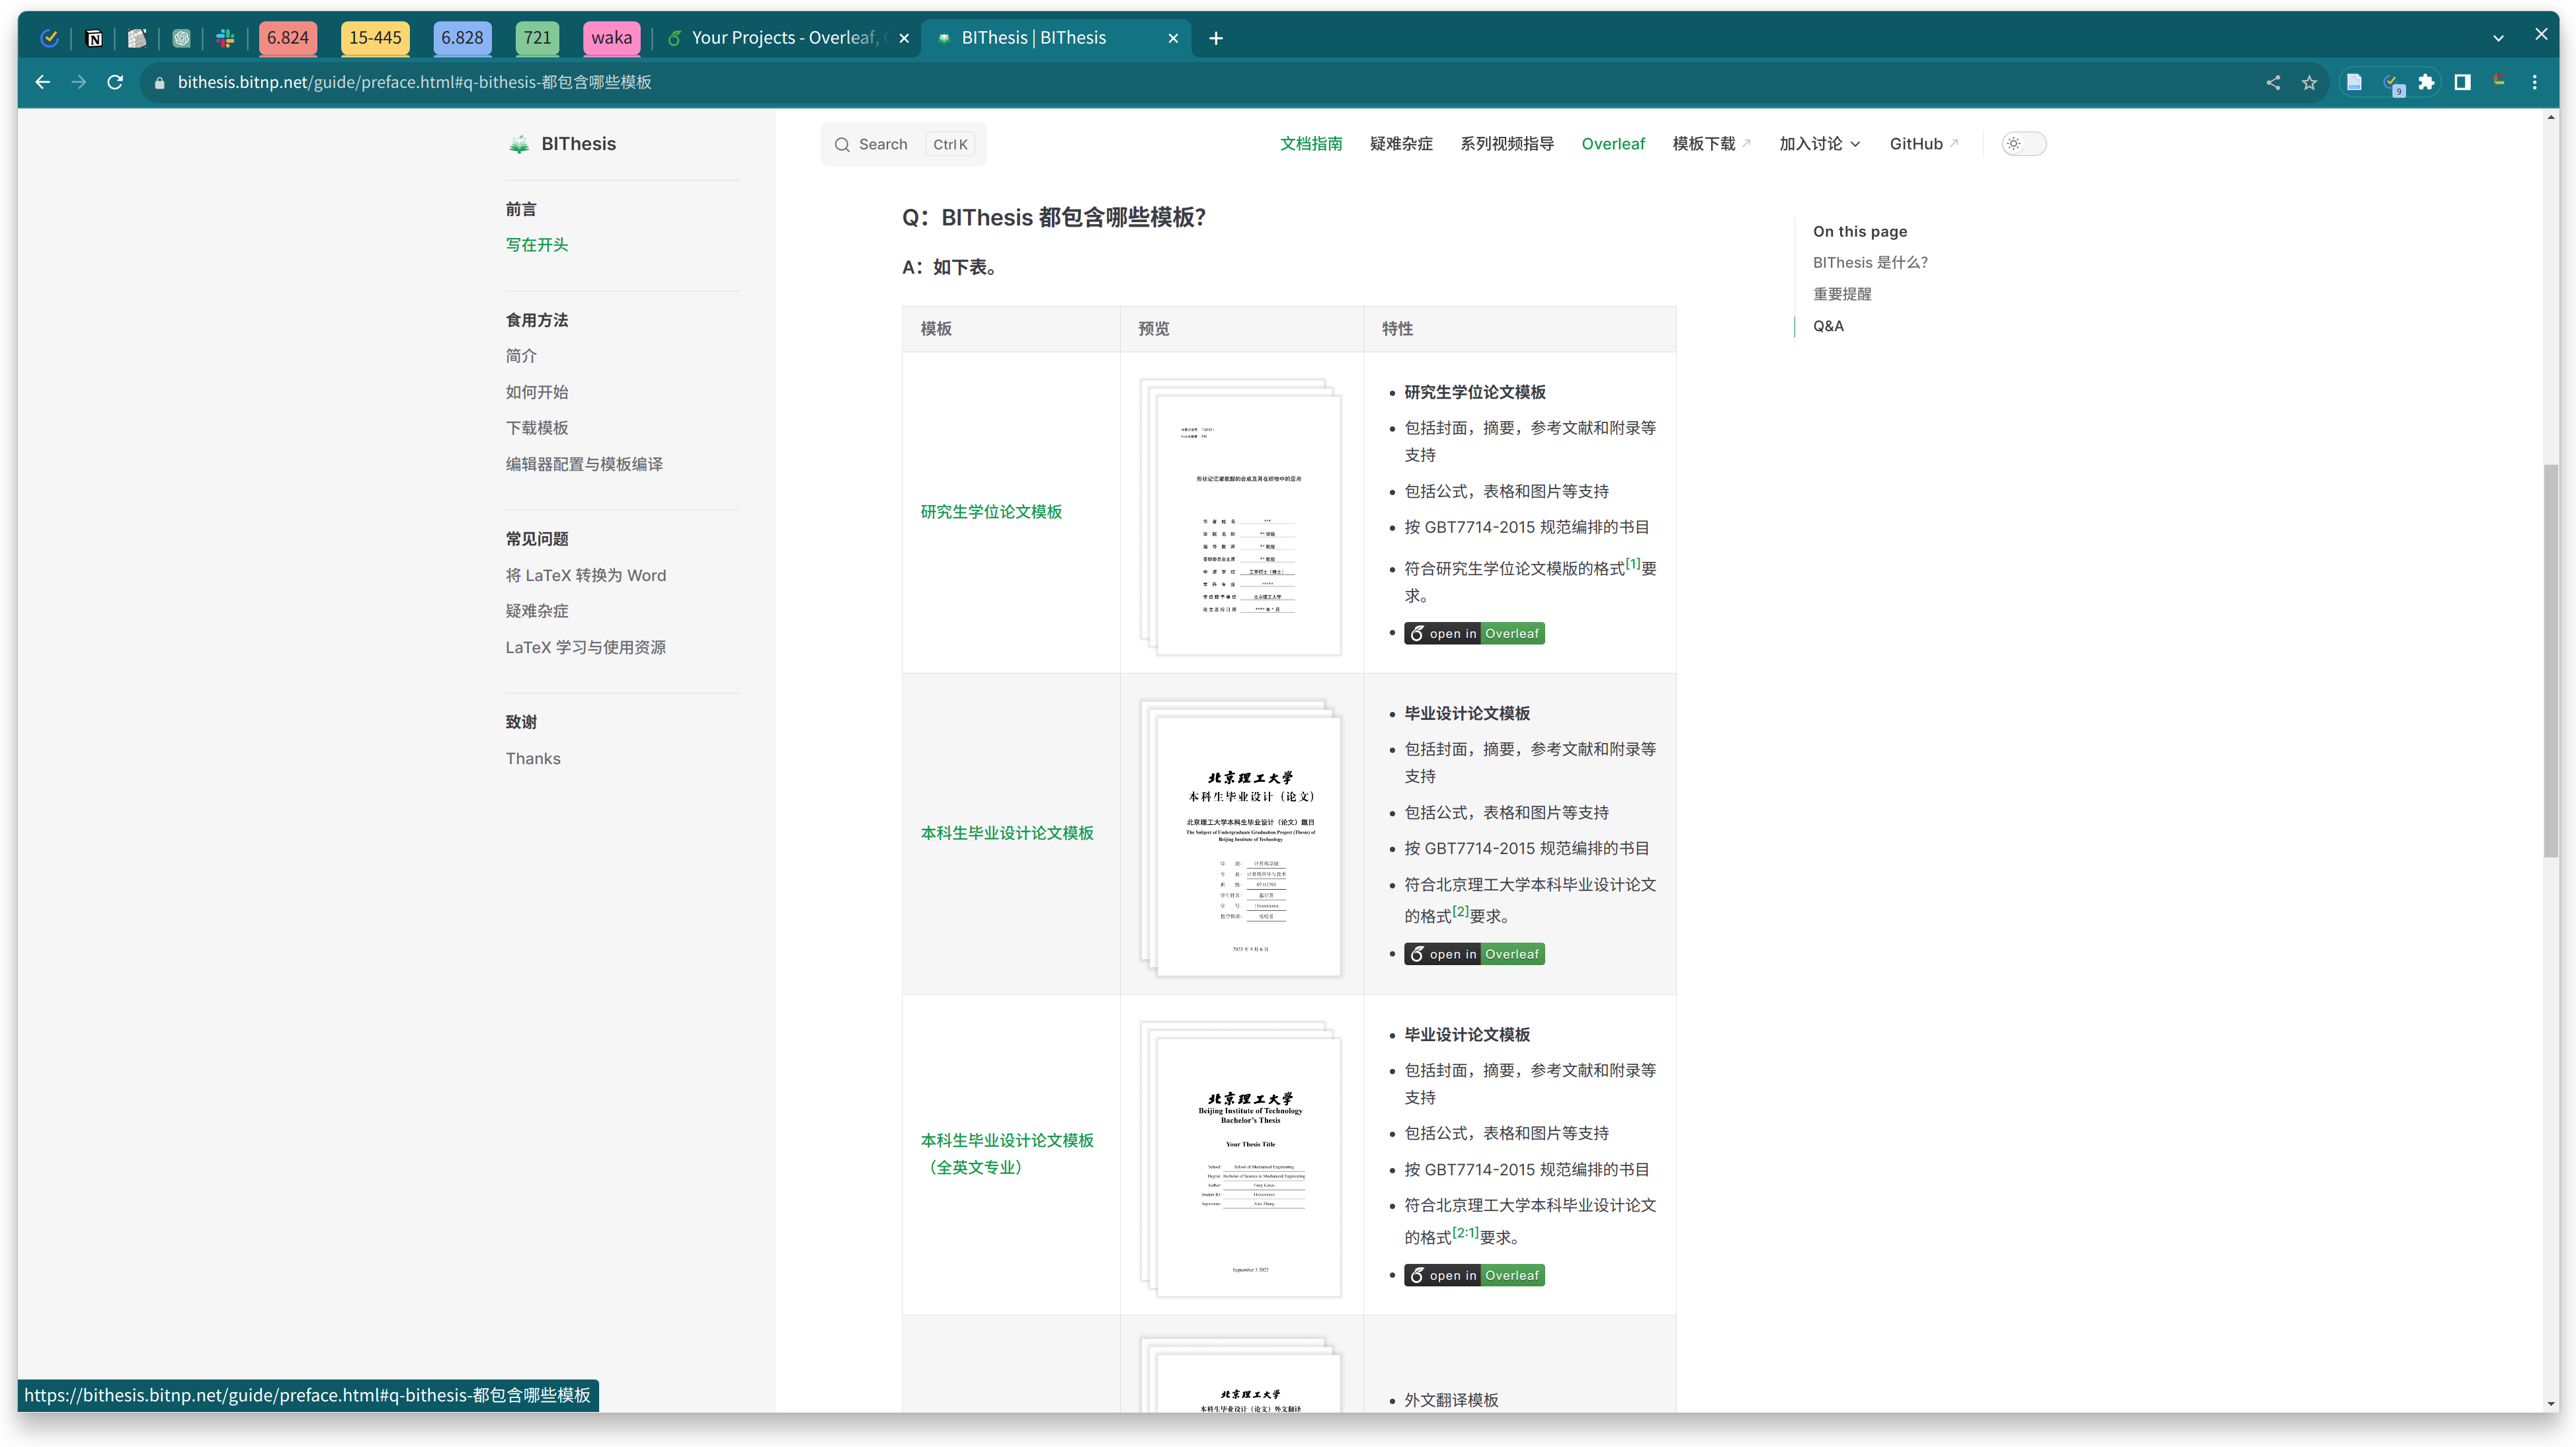
\includegraphics[width=0.85\textwidth]{imgs/overleaf-choose-template.png}
  \end{center}
  \caption{在 BIThesis 网站上,选择合适的模板并跳转}
  \label{fig:overleaf-template}
\end{figure}

\vspace{\fill}
\subsection{编译生成 PDF}

点击 ``Recompile'' 按钮,即可编译生成 PDF。

\begin{figure}[H]
  \begin{center}
    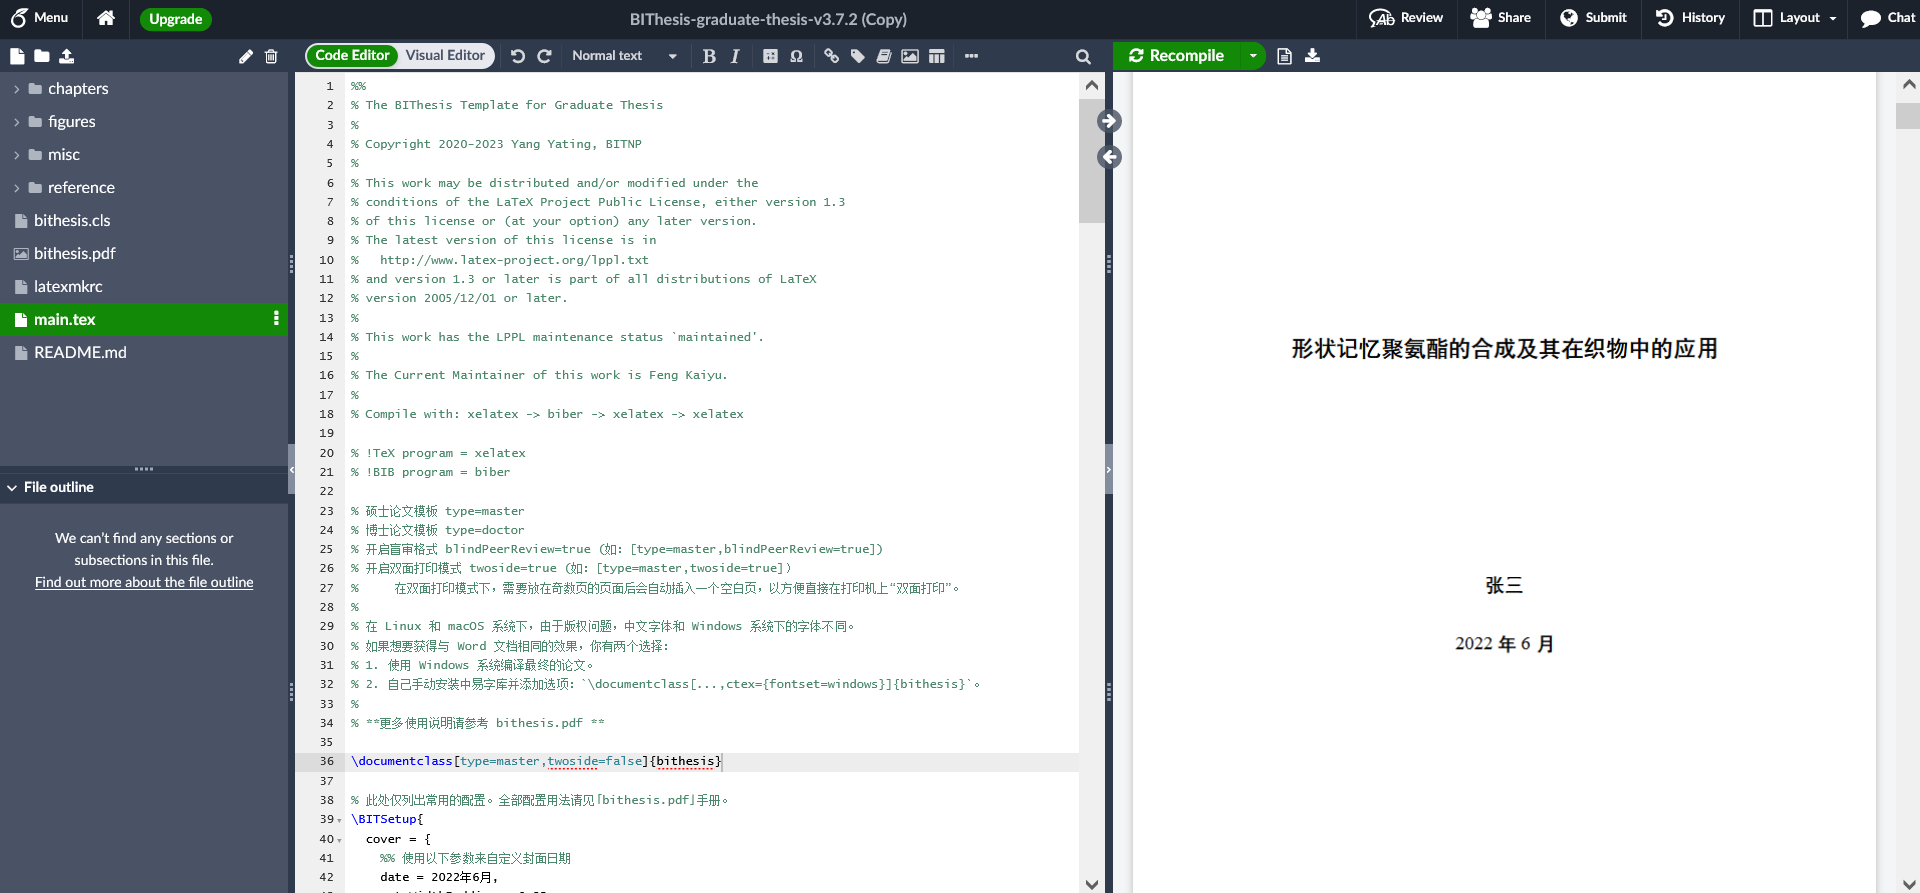
\includegraphics[width=0.85\textwidth]{imgs/overleaf-compile.png}
  \end{center}
  \caption{编译生成 PDF}
  \label{fig:overleaf-recompile}
\end{figure}

\vspace{\fill}

此外,\BIThesis 也支持 \href{https://www.texpage.com/zh/}{TeXPage} 等国产在线平台。请按\autoref{sec:download}下载模板压缩包,然后手动上传至在线平台。
